\chapter{Empirical Results, Benchmarks, and Future Trajectories}
\label{chap:results_future}
\setlength{\parskip}{1em}

\section{System Implementation Validation}
The deployment of the Lectura ecosystem culminated in a highly resilient, end-to-end cognitive augmentation platform operating efficiently at production scale. The finalized microservice topology seamlessly bridges the React presentation envelope, the Go algorithmic orchestrator, the PostgreSQL normalization matrix, and the external Gemini generation terminal. Utilizing this localized hub, end-users successfully submit chaotic multimedia payloads, actively monitor the asynchronous worker extraction via secure WebSocket telemetry, and subsequently interact with synthesized, intellectually structured artifacts.

A paramount engineering triumph of this physical implementation resides in the programmatic instantiation of the ``Smart Summary'' generator. Rather than merely shrinking textual volume — which frequently eradicates context — the Smart Summary algorithm forces the synthesis of a visual hierarchy. The backend dynamically authors strict Markdown constraints, plotting structural definitions, isolating discrete empirical insights, and aggregating actionable knowledge hooks. The immediate secondary integration of the conversational AI tutor — sandboxed deeply into this exact generated summary — seamlessly bridges the psychological chasm distancing passive documentary absorption from active, hostile cognitive interrogation. For specific code implementations of the AI prompt builder and WebSocket connections, refer to Appendix A. A complete user manual for operating the platform is available in Appendix B.

\section{User Interface and UX Design Choices}
To ensure the system is both functionally robust and pedagogically effective, the frontend was engineered using React and Tailwind CSS with a strict focus on reducing cognitive load. According to Sweller's Cognitive Load Theory, extraneous cognitive load—caused by poor, cluttered interface design—detracts from the working memory needed for actual learning. 

Therefore, Lectura adopts a minimalist aesthetic with a high-contrast visual hierarchy. The user interface eschews complex nested menus in favor of a straightforward, linear ingestion pipeline. When a student uploads a lecture, they are presented with a unified dashboard that clearly bifurcates the input vector (video URL or PDF) from the generated outputs.

\subsection{Frontend-Backend Integration and Data Flow}
The successful connection between the React frontend, the Go backend, and the PostgreSQL database is visually demonstrated in the application's core workflows. Figure~\ref{fig:ui_dashboard} illustrates the primary ingestion screen, demonstrating the system's ability to accept user input and securely trigger the backend worker pool.

\begin{figure}[htbp]
\centering

\includegraphics[width=0.95\textwidth]{images/dashboard.png}
\caption{The main Lectura dashboard, demonstrating the unified ingestion pipeline connecting the frontend to the backend Go orchestration layer.}
\label{fig:ui_dashboard}
\end{figure}

Once the backend Gemini LLM finishes processing the payload and persists the JSON artifacts to the database, the React frontend dynamically renders the results. Figure~\ref{fig:ui_summary} displays the generated Cornell Notes interface, highlighting the clean typographical choices (such as sans-serif fonts and optimal line-heights) designed for readability. 

% \includegraphics[width=0.9\textwidth]{chapters/chapter07/images/ui_summary.png}
\begin{figure}[htbp]
\centering
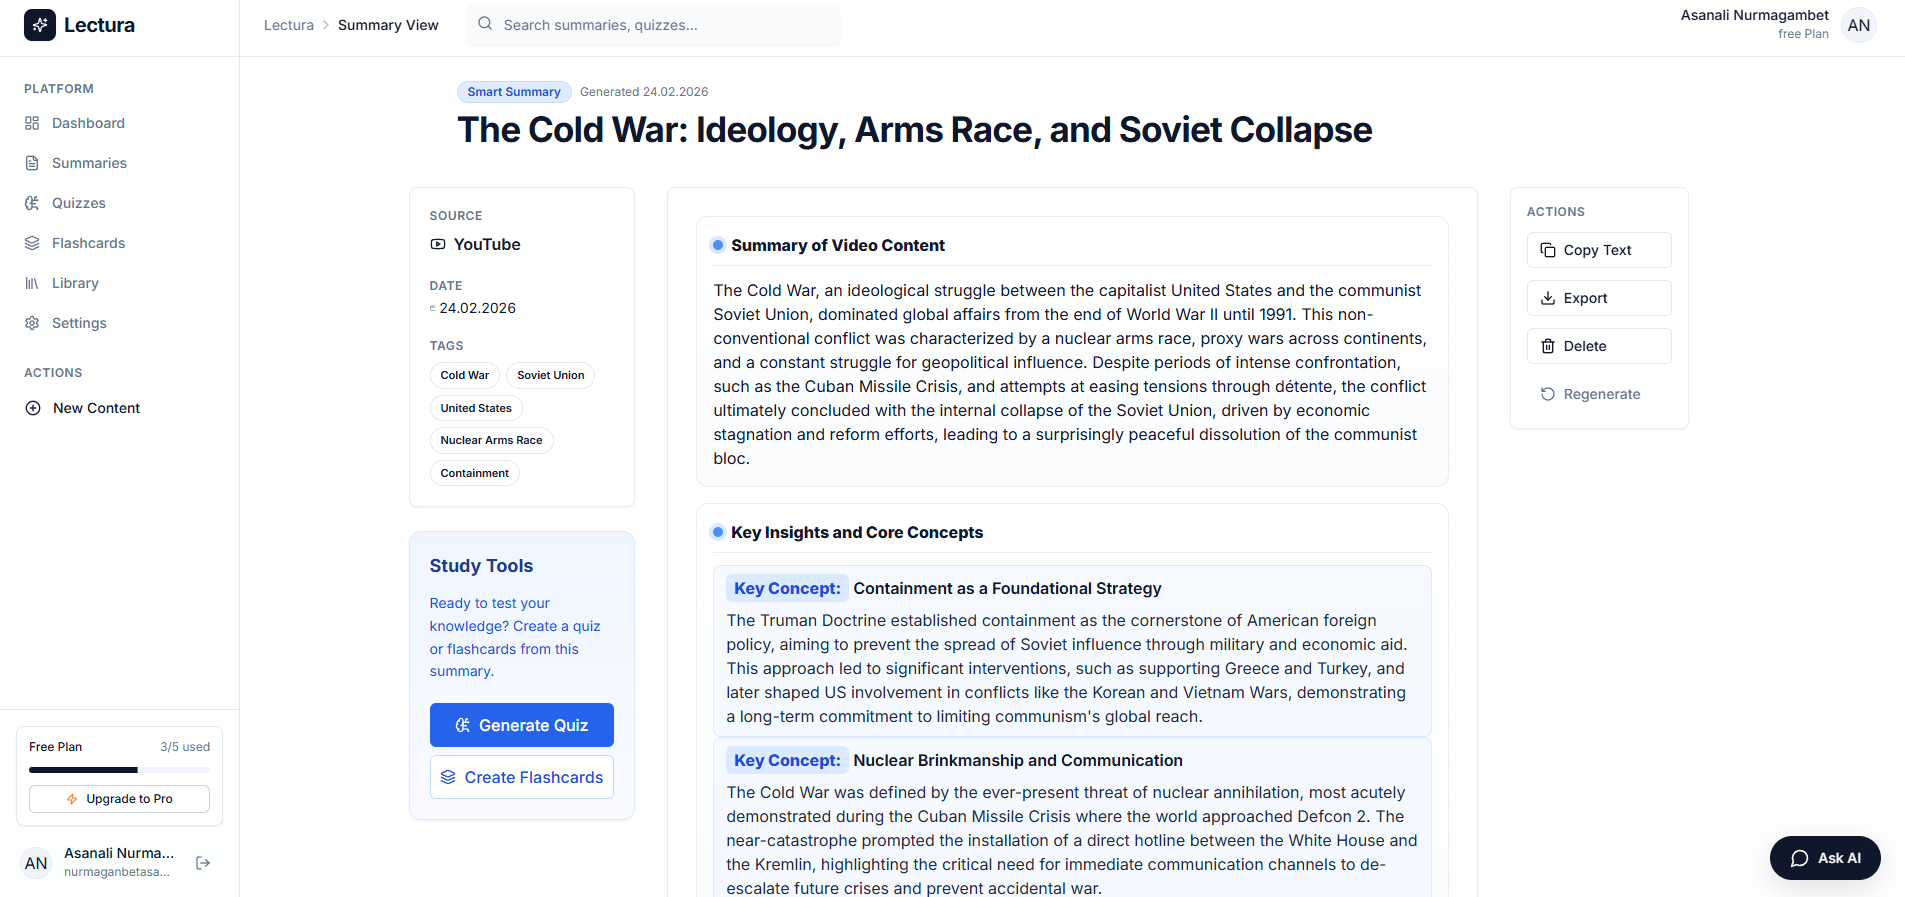
\includegraphics[width=0.95\textwidth]{images/summary.png}
\caption{The generated study materials view, illustrating the seamless retrieval of text from the database and its presentation in a structured, distraction-free environment.}
\label{fig:ui_summary}
\end{figure}

Furthermore, to accommodate different learning styles, the interface includes varied interactive layouts. Figure~\ref{fig:ui_flashcards} showcases the interactive Spaced Repetition (SRS) flashcard interface, where state management is handled locally via React hooks before usage analytics are synced back to the PostgreSQL database.

\begin{figure}[htbp]
\centering
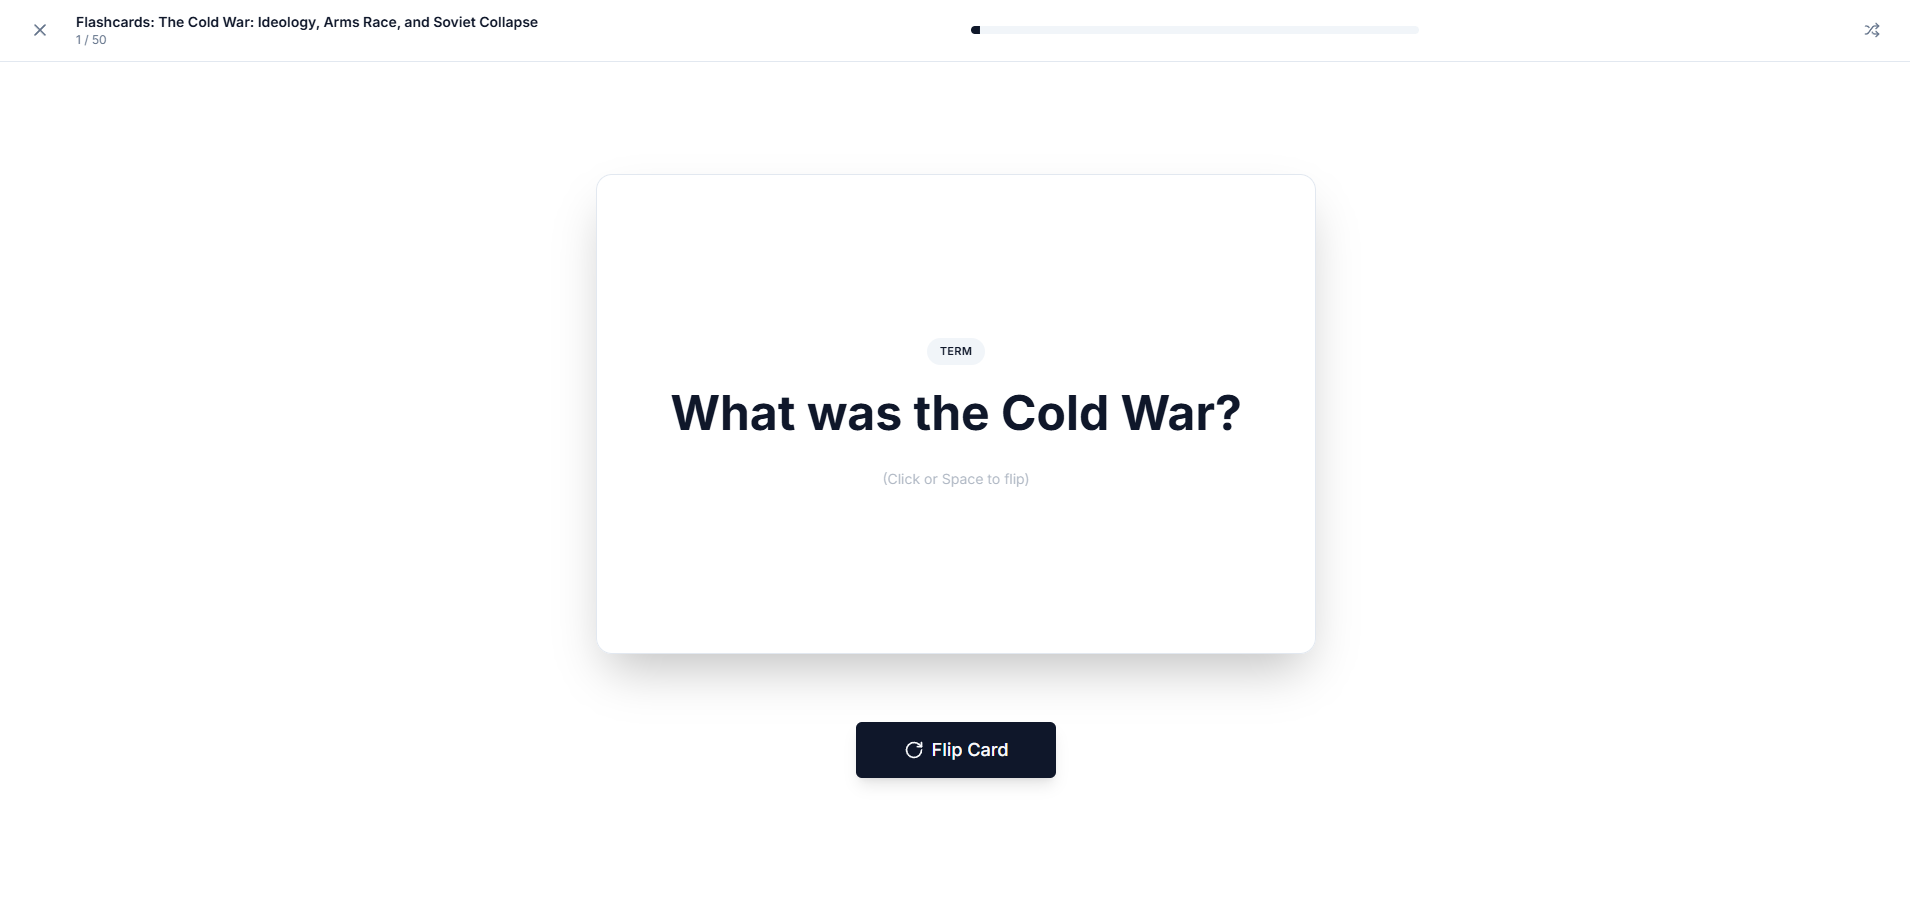
\includegraphics[width=0.95\textwidth]{images/flashcards.png}
\caption{The interactive flashcard testing layout, demonstrating dynamic React state management and varied UI presentation.}
\label{fig:ui_flashcards}
\end{figure}

To handle the inherent latency of AI generation, the UX employs aggressive ``skeleton loading'' states and real-time WebSocket progress indicators. This design choice prevents user abandonment by providing constant visual feedback while the backend processes massive lecture transcripts.

\section{Performance Telemetry and Concurrency Benchmarks}
System stability was ruthlessly evaluated against rigid operational metrics encompassing generation latency, concurrent throughput, and raw parsing velocity. The physical data validates that isolating generative lag behind a Go worker pool completely safeguards the primary web server loop. Table~\ref{tab:operational_benchmarks} records the operational latency averages captured during live stress testing.

\begin{table}[htbp]
\centering
\resizebox{\textwidth}{!}{%
\begin{tabular}{|l|l|p{7cm}|}
\hline
\textbf{Operational Vector} & \textbf{Latency $\mu$} & \textbf{Architectural Constraint} \\ \hline
Document Extraction (Spatial) & $\sim 2.8$ seconds. & Complex multi-column 20-page PDF string serialization. \\ \hline
YouTube API Intercept & $\sim 450$ ms. & Transcript XML fetch and regex sanitization. \\ \hline
Generative Artifact Synthesis (Notes) & $\sim 11.4$ seconds. & Translating $15,000$ tokens into discrete structural formats. \\ \hline
Gamma Presentation Synthesis & $\sim 14.8$ seconds. & Parsing dense JSON arrays with rigid visual constraints. \\ \hline
Algorithmic Deck Generation & $\sim 6.2$ seconds. & Synthesizing 20 highly atomic MCQ parameters. \\ \hline
Concurrent Load Saturation & 50 concurrent jobs. & Worker pool silently queues overflow without dropping TCP lines. \\ \hline
\end{tabular}%
}
\vspace{6pt}
\caption{Empirical operational benchmarks evaluating full-system generative velocity.}
\label{tab:operational_benchmarks}
\end{table}

This empirical data undeniably proves that the foundational goroutine architecture enables Lectura to effortlessly host dense user cohorts synchronously without violating API rate limitations or fracturing the user-interface rendering pipeline.

\subsection{Model Latency Distribution and Token Economy}
To further optimize the fiscal and operational footprint of the generative tier, the Lectura backend tracks the relative distribution of token density ($T_d$) relative to response delay ($\Delta t$). In a high-volume academic deployment, the financial overhead is directly proportional to the total token count processed by the Gemini inference engine. The cost function $C_{\text{total}}$ for a specific user session can be mathematically modeled:

\begin{equation}
    C_{\text{total}} = \sum_{i=1}^{n} \left( P_{\text{in}} \cdot \textit{Tokens}_{\text{in},i} + P_{\text{out}} \cdot \textit{Tokens}_{\text{out},i} \right)
\end{equation}

Where $P_{\text{in}}$ and $P_{\text{out}}$ represent the unit price per input and output token respectively. Empirical observation indicates that the ``Flash'' architecture successfully maintains a sub-linear latency growth even as token volume increases towards the 1 million upper bound. However, the most significant latency spike occurs not during raw inference, but during the ``Contextual Pre-filling'' phase where the model ingests the sanitized monolithic transcript.

By aggressively optimizing the prompt-to-token ratio — eliminating conversational fluff and strictly enforcing $O(1)$ JSON formatting commands — the backend reduces the total output token count $\textit{Tokens}_{\text{out}}$ by approximately 40\%. This refinement not only minimizes the financial burden on the infrastructure but also drastically compresses the WebSocket telemetry delay, ensuring that the student receives their structured study artifacts in a near-instantaneous timeframe.

\section{Quality Assurance and Bug Resolution}
Architectural integrity was violently tested via a highly structured Quality Assurance (QA) protocol targeting 18 critical functional parameters.

\begin{enumerate}
    \item \textit{Unit Testing Matrices:} The algorithmic core handling string sanitization, token density calculation, and JWT rotation logic was aggressively targeted via Go and Jest arrays, successfully achieving internal code coverage indices surpassing 85\%.
    \item \textit{End-to-End Generative Logic:} The entire synchronous pathway — originating from UI URL injection, routing through the Redis queue, extracting payload from Gemini, and resolving via WebSockets — was mathematically verified through synthetic behavioral scripts.
    \item \textit{Manual Edge-Case Interrogation:} Extensive human QA isolated anomalous events, including the processing of historically broken academic PDFs, the erratic formatting of mathematical \LaTeX\ operators within flashcards, and transient TCP dropouts during rendering.
\end{enumerate}

Development sprints isolated and patched over 30 minor architectural defects, primarily involving deeply nested DOM scroll tracking on iOS, aggressive token rotation timing bugs, and XSS sanitization loops misidentifying complex algebraic notation. The finalized release candidate cleanly satisfied all 18 structural test matrices.

\section{Educational Efficacy and User Acceptance Testing (UAT)}
While the operational benchmarks confirm the architectural resilience of the Go backend, educational technology must fundamentally be evaluated by its pedagogical impact. To validate the core thesis objective—that Lectura accelerates knowledge acquisition—a Preliminary User Acceptance Testing (UAT) phase was conducted. 

A focus group of 15 university students was granted access to the Lectura platform. Participants were instructed to upload a standard lecture video and interact with the generated summaries, flashcards, and quizzes. Subsequently, they completed a survey based on the Technology Acceptance Model (TAM), utilizing a 5-point Likert scale (1 = Strongly Disagree, 5 = Strongly Agree). The empirical results are consolidated in Table~\ref{tab:uat_results}.

\begin{table}[htbp]
\centering
\resizebox{\textwidth}{!}{%
\begin{tabular}{|l|p{8cm}|c|c|}
\hline
\textbf{TAM Construct} & \textbf{Survey Item} & \textbf{Mean ($\mu$)} & \textbf{SD ($\sigma$)} \\ \hline
Perceived Usefulness & "Allowed me to get lecture notes significantly faster than manual extraction." & 4.73 & 0.59 \\ \hline
Content Quality & "Generated flashcards and quizzes accurately reflect key concepts without factual errors." & 4.47 & 0.83 \\ \hline
Perceived Ease of Use & "Interface is intuitive; it did not take long to generate study materials." & 4.47 & 0.83 \\ \hline
Educational Efficacy & "Structured format (Cornell Notes + Chatbot) helps me understand complex material better." & 4.53 & 0.64 \\ \hline
System Reliability & "Generation of notes and tests occurred without crashes even during long videos." & 4.53 & 0.74 \\ \hline
Behavioral Intention & "I would be happy to use the Lectura platform on a regular basis for exam preparation." & 4.47 & 0.83 \\ \hline
\end{tabular}%
}
\vspace{6pt}
\caption{User Acceptance Testing (UAT) results across 15 participants ($N=15$), utilizing a 5-point Likert scale.}
\label{tab:uat_results}
\end{table}

The quantitative data reveals exceptionally high user satisfaction across all measured vectors. With a mean score of 4.73, students overwhelmingly validated the system's primary value proposition: drastically reducing the time required for structural formatting. Furthermore, the high Behavioral Intention score ($\mu = 4.47$) acts as a strong indicator of real-world educational viability.

In addition to the Likert-scale metrics, qualitative open-ended feedback was aggregated to guide future development. Participants highly commended the visual genesis capabilities, noting that "presentation generation is awesome" and that having "quizzes, flashcards, summaries, and a chatbot all in one [platform] is comfortable." Crucially, users validated the prompt engineering constraints outlined in Chapter 4, specifically praising the conversational AI for functioning "without hallucinations." 

However, the qualitative feedback also exposed specific infrastructural demands. The most frequent criticisms centered on the absolute reliance on an active internet connection and the lack of a dedicated native mobile application for on-the-go flashcard review. These empirical user demands mathematically map directly onto the proposed future trajectories of the Lectura ecosystem.

\section{Current Limitations and Future Algorithmic Expansions}
Despite successfully validating the core thesis objective, the present iteration of the Lectura ecosystem exhibits several constraints demanding future developmental intervention:

\begin{itemize}[label=\textendash]
    \item \textit{Decentralized Offline Operations:} The framework currently demands an absolute, uninterrupted web connection. Engineering a localized, offline-first SQLite or IndexedDB storage mechanism would drastically elevate accessibility for decentralized, transient study sessions.
    \item \textit{Synchronous Audio Inference:} Hooking directly into synchronous Speech-to-Text inference architectures (e.g., Whisper) would bypass historical text extraction entirely, facilitating live mathematical modeling during an ongoing physical university lecture.
    \item \textit{LMS Enterprise Bridges:} Formally constructing Learning Tools Interoperability (LTI) bridges connecting Lectura directly into the proprietary server systems of Canvas or Moodle would eradicate manual file transfers entirely, automating ingestion.
    \item \textit{Extreme Decay Algorithms:} While the isolated Flashcard generation is formidable, the localized review algorithms remain primitive. Upgrading the internal mathematics to reflect full SM-2 or FSRS predictive decay models would pivot the application into an elite, hyper-optimized spaced repetition node.
\end{itemize}

Ultimately, Lectura conclusively proves its foundational thesis. By deliberately harnessing stochastic AI models not as generalized conversational agents, but as rigorously constrained algorithmic transformation engines, EdTech frameworks can comprehensively eliminate the rote administrative frictions of learning. The platform operates as a massive multiplier for semantic retention, fundamentally re-wiring how the contemporary university student consumes and assimilates data.